\subsection{System}
Ein System besteht aus mehreren Einzelgeräten, mit welchen, wie vorhin beschrieben, das Zählen, die Kategorisierung und die Geschwindigkeitsmessung durchgeführt werden. Es werden mehrere Geräte benötigt um den Verkehrsfluss in dem definiert begrenztem Gebiet darstellen zu können. Dabei werden die über den aufgenommenen Zeitstempel und die Fahrtrichtung der Verkehrsfluss statistisch rekonstruiert. Hierbei wird das vorhin erstellte Netzwerk des begrenzten Gebietes als Darstellungsgrundlage verwendet. Es werden zunächst die nächstgelegenen Geräte, welche auf direktem Weg erreichbar sind, identifiziert und von diesen die Daten des Feature Vektors extrahiert. Diese Daten werden dann nach dem Zeitstempel sortiert und mit einem Index versehen. Sind die Daten nun vorbereitet werden durch die Länge der Verbindungen und Geschwindigkeiten auf diesen, die voraussichtliche Durchfahrtszeit berechnet. Danach wird statistisch die höchste Wahrscheinlichkeit welchen Weg der Verkehrsteilnehmer nahm berechnet und eingezeichnet. Sind alle Geräte untereinander verglichen und alle Wege in dem Netzwerk eingezeichnet sind erhält man, wie unten dargestellt (\fref{bAuswertung}), eine Auswertung. 

\begin{figure}[H]
  \centering
  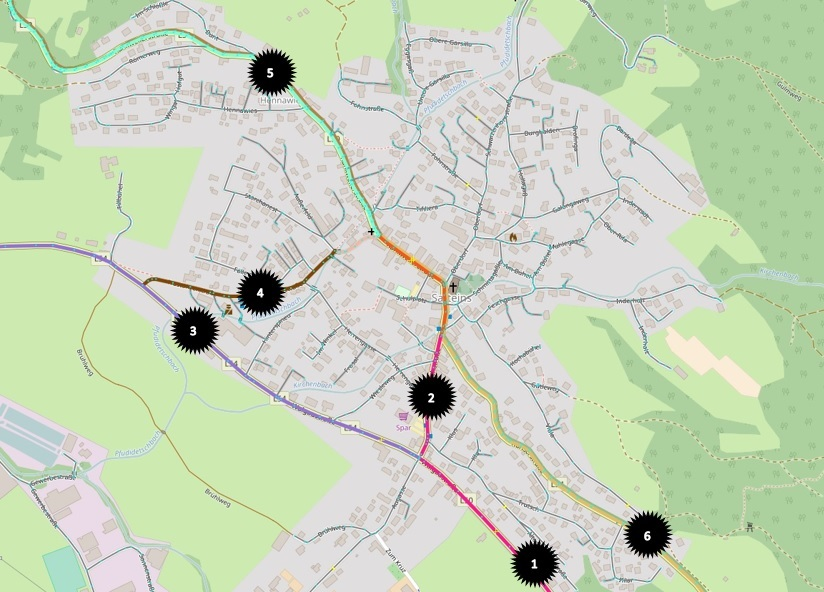
\includegraphics[width=0.6\textwidth]{Resultate/Auswertung.jpg} 
  \caption{Darstellung des Verkehrsflusses in Satteins.}
  \label{bAuswertung}
\end{figure}
In \tref{tVerkehrsfluss} ist der Verkehrsfluss von jedem Gerät zu seinem direkten Nachfolger tabellarisch dargestellt. 

\setlength\tabcolsep{5pt}

\begin{table}[H]
\centering
\begin{tabular}{|p{1.5cm}|p{1.5cm}|p{1.5cm}|p{1.5cm}|p{1.5cm}|p{1.5cm}|p{1.5cm}|p{1.5cm}|}
\hline
	von/nach & 1 & 2 & 3 & 4 & 5 & 6 & Out \\ \hline
	1 &  & 952 & 949 &  &  &  & 1703 \\ \hline
	2 & 326 & 0 & 279 & 105 & 434 & 275 & 0 \\ \hline
	3 & 996 & 0 &  &  &  &  & 1468 \\ \hline
	4 &  & 149 &  &  & 105 & 84 & 520 \\ \hline
	5 &  & 723 &  & 159 & 521 & 224 & 1668 \\ \hline
	6 &  & 313 &  & 78 & 426 &  & 327 \\ \hline
\end{tabular}
\caption{Tabelarische Darstellung des Verkehrsflusses.}
\label{tVerkehrsfluss}
\end{table}

\setlength\tabcolsep{0pt}